\documentclass[tikz, border=20pt]{standalone}
\usetikzlibrary{shapes.geometric, arrows.meta, positioning, calc, fit, backgrounds}

\begin{document}
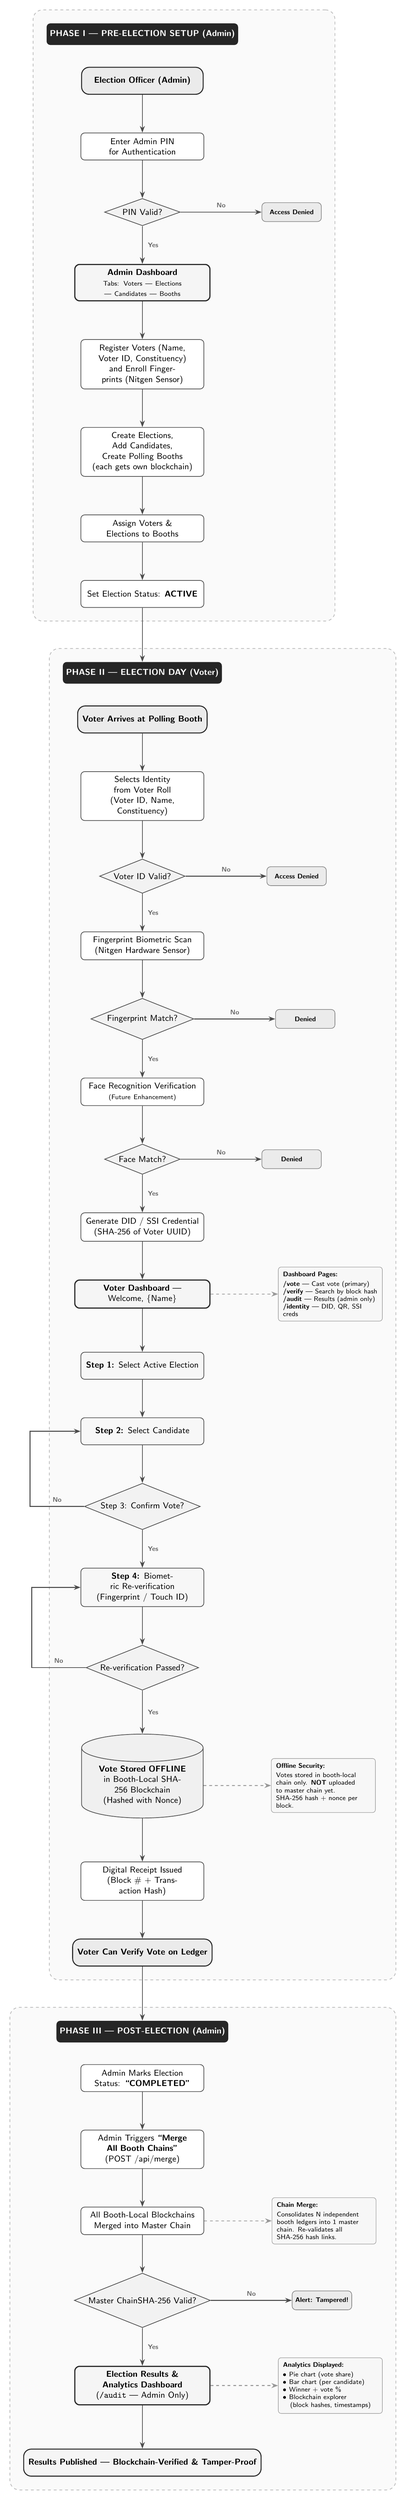
\begin{tikzpicture}[
    % ── Node Styles ──
    startstop/.style={
        rectangle, rounded corners=8pt,
        minimum width=4.5cm, minimum height=1cm,
        text centered, draw=black!85, line width=1pt,
        fill=black!8, font=\sffamily\small\bfseries,
        inner sep=5pt
    },
    process/.style={
        rectangle, rounded corners=4pt,
        minimum width=4.5cm, minimum height=1cm,
        text centered, draw=black!70, line width=0.7pt,
        fill=white, font=\sffamily\small,
        text width=4.2cm, inner sep=5pt
    },
    decision/.style={
        diamond, aspect=2.5,
        minimum width=2.8cm,
        text centered, draw=black!70, line width=0.7pt,
        fill=black!5, font=\sffamily\small,
        inner sep=2pt
    },
    database/.style={
        cylinder, shape border rotate=90, aspect=0.25,
        minimum width=4.5cm, minimum height=1.2cm,
        text centered, draw=black!70, line width=0.7pt,
        fill=black!6, font=\sffamily\small,
        text width=3.8cm, inner sep=4pt
    },
    dashbox/.style={
        rectangle, rounded corners=5pt,
        minimum width=5cm, minimum height=1cm,
        text centered, draw=black!85, line width=1.2pt,
        fill=black!4, font=\sffamily\small,
        text width=4.6cm, inner sep=5pt
    },
    rejected/.style={
        rectangle, rounded corners=4pt,
        minimum width=2.2cm, minimum height=0.7cm,
        text centered, draw=black!50, line width=0.6pt,
        fill=black!8, font=\sffamily\scriptsize\bfseries
    },
    phaselabel/.style={
        rectangle, rounded corners=4pt,
        minimum width=5.5cm, minimum height=0.8cm,
        text centered, fill=black!85, text=white,
        font=\sffamily\small\bfseries
    },
    sideinfo/.style={
        rectangle, rounded corners=3pt,
        draw=black!40, line width=0.5pt,
        fill=black!3, font=\sffamily\scriptsize,
        text width=3.5cm, inner sep=5pt, align=left
    },
    % ── Arrow Styles ──
    arrow/.style={-Stealth, line width=0.9pt, draw=black!70},
    nolabel/.style={font=\sffamily\scriptsize\bfseries, text=black!60},
    yeslabel/.style={font=\sffamily\scriptsize\bfseries, text=black!60},
]


% ════════════════════════════════════════════════════════════
%  PHASE I — PRE-ELECTION SETUP
% ════════════════════════════════════════════════════════════

\node (P1) [phaselabel] {PHASE I \textemdash\ PRE-ELECTION SETUP (Admin)};

\node (A1) [startstop, below=0.8cm of P1]
    {Election Officer (Admin)};

\node (A2) [process, below=1.4cm of A1]
    {Enter Admin PIN for Authentication};

\node (A3) [decision, below=1.4cm of A2]
    {PIN Valid?};
\node (A3no) [rejected, right=3cm of A3] {Access Denied};

\node (A4) [dashbox, below=1.4cm of A3]
    {\textbf{Admin Dashboard}\\{\scriptsize Tabs: Voters | Elections | Candidates | Booths}};

\node (A5) [process, below=1.4cm of A4]
    {Register Voters (Name, Voter ID, Constituency)\\and Enroll Fingerprints (Nitgen Sensor)};

\node (A6) [process, below=1.4cm of A5]
    {Create Elections, Add Candidates,\\Create Polling Booths (each gets own blockchain)};

\node (A7) [process, below=1.4cm of A6]
    {Assign Voters \& Elections to Booths};

\node (A8) [process, below=1.4cm of A7]
    {Set Election Status: \textbf{ACTIVE}};

% Phase I arrows — all vertical, guaranteed zero overlaps
\draw [arrow] (A1) -- (A2);
\draw [arrow] (A2) -- (A3);
\draw [arrow] (A3) -- node[yeslabel, right=2pt] {Yes} (A4);
\draw [arrow] (A3) -- node[nolabel, above=1pt] {No} (A3no);
\draw [arrow] (A4) -- (A5);
\draw [arrow] (A5) -- (A6);
\draw [arrow] (A6) -- (A7);
\draw [arrow] (A7) -- (A8);


% ════════════════════════════════════════════════════════════
%  PHASE II — ELECTION DAY (VOTER)
% ════════════════════════════════════════════════════════════

\node (P2) [phaselabel, below=2.0cm of A8]
    {PHASE II \textemdash\ ELECTION DAY (Voter)};

\node (B1) [startstop, below=0.8cm of P2]
    {Voter Arrives at Polling Booth};

\node (B2) [process, below=1.4cm of B1]
    {Selects Identity from Voter Roll\\(Voter ID, Name, Constituency)};

\node (B3) [decision, below=1.4cm of B2]
    {Voter ID Valid?};
\node (B3no) [rejected, right=3cm of B3] {Access Denied};

\node (B4) [process, below=1.4cm of B3]
    {Fingerprint Biometric Scan\\(Nitgen Hardware Sensor)};

\node (B5) [decision, below=1.4cm of B4]
    {Fingerprint Match?};
\node (B5no) [rejected, right=3cm of B5] {Denied};

\node (B6) [process, below=1.4cm of B5]
    {Face Recognition Verification\\{\scriptsize (Future Enhancement)}};

\node (B7) [decision, below=1.4cm of B6]
    {Face Match?};
\node (B7no) [rejected, right=3cm of B7] {Denied};

\node (B8) [process, below=1.4cm of B7]
    {Generate DID / SSI Credential\\(SHA-256 of Voter UUID)};

\node (B9) [dashbox, below=1.4cm of B8]
    {\textbf{Voter Dashboard} \textemdash\ Welcome, \{Name\}};

% Side info: Dashboard pages
\node (B9info) [sideinfo, right=2.5cm of B9] {
    \textbf{Dashboard Pages:}\\[2pt]
    \textbf{/vote} \textemdash\ Cast vote (primary)\\
    \textbf{/verify} \textemdash\ Search by block hash\\
    \textbf{/audit} \textemdash\ Results (admin only)\\
    \textbf{/identity} \textemdash\ DID, QR, SSI creds
};

% Phase II arrows — all vertical or rightward
\draw [arrow] (A8) -- (P2);
\draw [arrow] (B1) -- (B2);
\draw [arrow] (B2) -- (B3);
\draw [arrow] (B3) -- node[yeslabel, right=2pt] {Yes} (B4);
\draw [arrow] (B3) -- node[nolabel, above=1pt] {No} (B3no);
\draw [arrow] (B4) -- (B5);
\draw [arrow] (B5) -- node[yeslabel, right=2pt] {Yes} (B6);
\draw [arrow] (B5) -- node[nolabel, above=1pt] {No} (B5no);
\draw [arrow] (B6) -- (B7);
\draw [arrow] (B7) -- node[yeslabel, right=2pt] {Yes} (B8);
\draw [arrow] (B7) -- node[nolabel, above=1pt] {No} (B7no);
\draw [arrow] (B8) -- (B9);
\draw [arrow, dashed, draw=black!40] (B9) -- (B9info);


% ════════════════════════════════════════════════════════════
%  VOTING SUB-FLOW
% ════════════════════════════════════════════════════════════

\node (C1) [process, below=1.6cm of B9, fill=black!3]
    {\textbf{Step 1:} Select Active Election};

\node (C2) [process, below=1.4cm of C1, fill=black!3]
    {\textbf{Step 2:} Select Candidate};

\node (C3) [decision, below=1.4cm of C2]
    {Step 3: Confirm Vote?};

\node (C4) [process, below=1.4cm of C3, fill=black!3]
    {\textbf{Step 4:} Biometric Re-verification\\(Fingerprint / Touch ID)};

\node (C5) [decision, below=1.4cm of C4]
    {Re-verification Passed?};

\node (C6) [database, below=1.6cm of C5]
    {\textbf{Vote Stored OFFLINE}\\in Booth-Local SHA-256 Blockchain\\(Hashed with Nonce)};

\node (C7) [process, below=1.6cm of C6]
    {Digital Receipt Issued\\(Block \# + Transaction Hash)};

\node (C8) [startstop, below=1.4cm of C7]
    {Voter Can Verify Vote on Ledger};

% Side info: Offline storage note
\node (C6info) [sideinfo, right=2.5cm of C6] {
    \textbf{Offline Security:}\\[2pt]
    Votes stored in booth-local\\
    chain only. \textbf{NOT} uploaded\\
    to master chain yet.\\
    SHA-256 hash + nonce per block.
};

% Voting arrows — all vertical
\draw [arrow] (B9) -- (C1);
\draw [arrow] (C1) -- (C2);
\draw [arrow] (C2) -- (C3);
\draw [arrow] (C3) -- node[yeslabel, right=2pt] {Yes} (C4);
\draw [arrow] (C4) -- (C5);
\draw [arrow] (C5) -- node[yeslabel, right=2pt] {Yes} (C6);
\draw [arrow] (C6) -- (C7);
\draw [arrow] (C7) -- (C8);
\draw [arrow, dashed, draw=black!40] (C6) -- (C6info);

% Loopbacks — routed via LEFT gutter, no box crossings
\draw [arrow] (C3.west) -- ++(-2, 0) node[nolabel, above=1pt, midway] {No} |- (C2.west);
\draw [arrow] (C5.west) -- ++(-2, 0) node[nolabel, above=1pt, midway] {No} |- (C4.west);


% ════════════════════════════════════════════════════════════
%  PHASE III — POST-ELECTION
% ════════════════════════════════════════════════════════════

\node (P3) [phaselabel, below=2.0cm of C8]
    {PHASE III \textemdash\ POST-ELECTION (Admin)};

\node (D1) [process, below=0.8cm of P3]
    {Admin Marks Election Status: \textbf{``COMPLETED''}};

\node (D2) [process, below=1.4cm of D1]
    {Admin Triggers \textbf{``Merge All Booth Chains''}\\(POST /api/merge)};

\node (D3) [process, below=1.4cm of D2]
    {All Booth-Local Blockchains\\Merged into Master Chain};

\node (D4) [decision, below=1.4cm of D3]
    {Master Chain\\SHA-256 Valid?};
\node (D4no) [rejected, right=3cm of D4] {Alert: Tampered!};

\node (D5) [dashbox, below=1.4cm of D4]
    {\textbf{Election Results \& Analytics Dashboard}\\(\texttt{/audit} \textemdash\ Admin Only)};

% Side info: Analytics detail
\node (D5info) [sideinfo, right=2.5cm of D5] {
    \textbf{Analytics Displayed:}\\[2pt]
    \textbullet\ Pie chart (vote share)\\
    \textbullet\ Bar chart (per candidate)\\
    \textbullet\ Winner + vote \%\\
    \textbullet\ Blockchain explorer\\
    \quad (block hashes, timestamps)
};

\node (D6) [startstop, below=1.6cm of D5, fill=black!4]
    {Results Published \textemdash\ Blockchain-Verified \& Tamper-Proof};

% Phase III arrows — all vertical or rightward
\draw [arrow] (C8) -- (P3);
\draw [arrow] (D1) -- (D2);
\draw [arrow] (D2) -- (D3);
\draw [arrow] (D3) -- (D4);
\draw [arrow] (D4) -- node[yeslabel, right=2pt] {Yes} (D5);
\draw [arrow] (D4) -- node[nolabel, above=1pt] {No} (D4no);
\draw [arrow] (D5) -- (D6);
\draw [arrow, dashed, draw=black!40] (D5) -- (D5info);

% Side info: Merge note
\node (D3info) [sideinfo, right=2.5cm of D3] {
    \textbf{Chain Merge:}\\[2pt]
    Consolidates N independent\\
    booth ledgers into 1 master\\
    chain. Re-validates all\\
    SHA-256 hash links.
};
\draw [arrow, dashed, draw=black!40] (D3) -- (D3info);


% ════════════════════════════════════════════════════════════
%  BACKGROUND PHASE BOXES
% ════════════════════════════════════════════════════════════
\begin{scope}[on background layer]
    \node[fit=(P1)(A1)(A3no)(A8),
          draw=black!25, dashed, line width=0.8pt, rounded corners=10pt,
          inner sep=14pt, fill=black!2] {};
    \node[fit=(P2)(B1)(B3no)(B5no)(B7no)(B9)(B9info)(C1)(C2)(C3)(C4)(C5)(C6)(C6info)(C7)(C8),
          draw=black!25, dashed, line width=0.8pt, rounded corners=10pt,
          inner sep=14pt, fill=black!2] {};
    \node[fit=(P3)(D1)(D4no)(D5)(D5info)(D3info)(D6),
          draw=black!25, dashed, line width=0.8pt, rounded corners=10pt,
          inner sep=14pt, fill=black!2] {};
\end{scope}

\end{tikzpicture}
\end{document}
